% book模板
% book模板.tex

\documentclass[12pt,UTF8]{ctexbook}

% 设置纸张信息。
\input{../../../common/page}

% 设置字体，并解决显示难检字问题。
\xeCJKsetup{AutoFallBack=true}
% 注意：ctexbook类已默认设置SimSun为CJKrmdefault
% 以下设置用于确保字体回退和扩展字体可用
% 仅设置扩展字体以避免与默认设置冲突
\setCJKfamilyfont{hei}{SimHei}
\setCJKfamilyfont{kai}{KaiTi}

% 目录 chapter 级别加点（.）。
\usepackage{titletoc}
\titlecontents{chapter}[0pt]{\vspace{3mm}\bf\addvspace{2pt}\filright}{\contentspush{\thecontentslabel\hspace{0.8em}}}{}{\titlerule*[8pt]{.}\contentspage}

% 支持目录点击跳转
\usepackage[colorlinks,linkcolor=blue,citecolor=blue,urlcolor=blue]{hyperref}

% 设置 part 和 chapter 标题格式。
\ctexset{
	part/name= {第,卷},
	part/number={\chinese{part}},
	chapter/name={第,篇},
	chapter/number={\arabic{chapter}}
}

% 图片相关设置。
\usepackage{graphicx}
\graphicspath{{Images/}}

% 设置署名格式。
\newenvironment{shuming}{\hfill\zihao{4}}

% 注脚每页重新编号，避免编号过大。
\usepackage[perpage]{footmisc}

% 设置古文原文格式。
\newenvironment{yuanwen}{\bfseries\zihao{4}}

% 设置段落间距
\setlength{\parskip}{0.8em plus 0.2em minus 0.1em}

% 列表格式支持，列表项向右偏移。
\usepackage{enumitem}

% 数学公式支持
\usepackage{amsmath}

\title{\heiti\zihao{0} 矿石收音机}
\author{}
\date{}

\begin{document}

\maketitle
\tableofcontents

\frontmatter
\chapter{前言}

矿石收音机是一种最简单、最经济的收音机，需用器材不多，制作容易，不需要维持费用；尤其是适合于在我国广大的农村中使用。这种简单而又经济的收音机，在装置上和检修上都不需要特殊的技术，最合于一般初学的无线电爱好者研究之用。

虽然矿石收音机也有它的缺点，如接收距离不远、声音小等，但是我国各省现在都已普遍设立了人民广播电台，故在很大的地区内，矿石收音机仍可使用。

\mainmatter

\chapter{无线电波的性质}

无线电广播是现代生活中不可或缺的一部分。通过收音机，我们可以听到新闻资讯、音乐娱乐、天气预报等各种节目。所有这些声音都是通过无线电波传递的。

无线电波和水的波浪十分相似，它们都是一种振动。我们在水面抛下一块石子，它就激起水的波浪——振动，一圈圈地向外扩散开去；如果水面正浮着一片树叶，它也就受到水波的影响而跟着上下浮动。广播进行时广播电台向四周发出无线电波，在电波作用的范围内，收音机就收到了同样的电波。

无线电波是一种电磁波。因为它可以不靠电线来传递，所以叫做"无线电波"。

\section{电磁波的产生}

电磁波是怎样发射出去的呢？要知道这个道理，首先得从电流说起。电流在电线里流动的方式有两种：一种叫"直流电"，电流流动的方向和大小都是一直不变的，像手电筒里的电池及其他各种干电池所产生的电流便是；另一种叫"交流电"，电流流动的方向是不停地来回变换，并且强度（即大小）也是忽大忽小变化的，城市中用来照明的电灯，绝大多数是使用交流电的。

电流在导线里面流动时能在导线周围产生电磁现象。性质不同的电流所产生的结果也是不同的，用以产生电磁波的是交流电流。

这种方向和强度不停变化的交流电，本质上是一种周期性的振荡。交流电的电压或电流随时间呈现规律性的变化。

交流电完成一次完整的周期性变化（即从零到正峰值，回到零，再到负峰值，最后回到零）所需的时间称为\textbf{周期}，常用符号$T$表示，单位是秒(s)。单位时间内（每秒）完成振荡的次数称为\textbf{频率}，常用符号$f$表示。根据国际单位制，频率的单位是\textbf{赫兹}（Hz），1 Hz表示每秒完成1次完整振荡。

在早期的无线电文献中，频率单位常写作"周"或"周/秒"（cycles per second，简称c.p.s.），其含义与赫兹完全相同：1周 = 1 Hz。例如旧文献中的"5周"即表示5 Hz，"500千周"即表示500 kHz（千赫兹）。这一用法在1960年第十一届国际计量大会正式采用"赫兹"作为标准单位名称后逐渐被取代，但在阅读20世纪中期的无线电技术资料时仍可能遇到。

频率与周期的关系为：

\begin{equation}
f = \frac{1}{T}
\end{equation}

例如，我国民用交流电的标准频率为50 Hz，意味着电流在1秒内完成50次完整周期性变化，对应的周期为0.02秒。而美国、日本部分地区则采用60 Hz的标准。

除了周期和频率之外，描述一个正弦交流电（或电磁波）还需要另一个关键参数——\textbf{振幅}。

\subsubsection{振幅}

\textbf{振幅}（Amplitude）是指振荡量偏离其平衡位置（零点）的最大值。对于交流电压而言，振幅就是电压从零上升到正向峰值的大小；对于交流电流而言，振幅就是电流达到的最大值。

以正弦交流电的数学表达式为例：

\begin{equation}
	v(t) = V_{m} \sin(2\pi f t + \phi)
\end{equation}

其中各参数含义如下：
\begin{itemize}
	\item $v(t)$ —— $t$时刻的瞬时电压值
	\item $V_{m}$ —— 电压\textbf{振幅}（最大值），单位为伏特(V)
	\item $f$ —— 频率，单位为赫兹(Hz)
	\item $\phi$ —— 初相位（决定$t=0$时刻的起始位置）
\end{itemize}

需要区分的是：振幅是\textbf{峰值}（最大值），而我们日常所说的"220V市电"指的是\textbf{有效值}（RMS值）。对于正弦波而言，有效值与振幅的关系为：

\begin{equation}
	V_{\text{rms}} = \frac{V_{m}}{\sqrt{2}} \approx 0.707 \, V_{m}
\end{equation}

因此，我国220V民用交流电的实际振幅约为 $220 \times \sqrt{2} \approx 311$ 伏特。\subsubsection{等幅波}

在描述交流电或电磁波时，还有一个重要概念——\textbf{等幅波}。

所谓\textbf{等幅波}（Constant Amplitude Wave / Continuous Wave, CW），是指在传播过程中振幅保持恒定不变的正弦波。换句话说，它的波形是一个"完美"的正弦曲线：每一周期的峰值高度完全相同，不会随时间忽大忽小。

等幅波可以用以下数学表达式描述：

\begin{equation}
	y(t) = A \sin(2\pi f t)
\end{equation}

其中$A$为恒定的振幅，不随时间变化。这种波形的特点是：
\begin{itemize}
	\item 振幅$A$始终为常数——波形"高度"均匀一致
	\item 只有频率$f$这一个变量来承载信息
	\item 在频谱上表现为一条单一的谱线（理想情况下）
\end{itemize}

\textbf{等幅波与调幅波的区别：}

在实际无线电通信中，为了传递声音等信息，需要对载波进行\textbf{调制}。最基本的方式之一就是调幅（AM，Amplitude Modulation）：

\begin{itemize}
	\item \textbf{等幅波（未调制载波）}：振幅恒定，仅用于传递摩尔斯电码等简单通断信号（如早期的无线电报）
	
	\item \textbf{调幅波（已调制信号）}：载波的振幅随音频信号的强弱而变化——声音大时振幅变大，声音小时振幅变小。矿石收音机接收的就是这类调幅广播信号
\end{itemize}

形象地理解：如果把等幅波比作一个人用\textbf{固定音量}持续唱同一个音调，那么调幅波就是这个人唱着\textbf{同样音调}但\textbf{音量时大时小}地在唱歌——音量的变化就携带了信息内容。

对于矿石收音机而言，它接收到的中波/短波信号正是经过音频调制的调幅波。矿石检波器的作用之一，就是将这种振幅的变化"提取"出来，还原成我们能够听到的音频信号。

\subsubsection{为什么需要调制？——音频电流的困境}

既然广播电台要传送的是声音信号，为什么不直接把音频电流发射出去呢？这就涉及到一个根本性的物理限制。

当我们说话或播放音乐时，声波会引起话筒（麦克风）中的膜片振动，通过电磁感应或压电效应将机械振动转换为电信号的振动——这就是所谓的\textbf{音频电流}或\textbf{低频电流}。人耳能感知的声音频率范围大约在20 Hz至20000 Hz（20 kHz）之间，因此音频电流的频率也处于这个低频范围内。

然而，正如前面所述，低频交流电\textbf{不能有效辐射电磁波}。原因在于：
\begin{itemize}
	\item 20 Hz--20 kHz的频率太低，根据电磁辐射理论，其辐射效率极低
	\item 即使能够发射出去，不同电台的音频信号频率范围高度重叠（都在20 Hz--20 kHz之间），接收端也无法区分来自不同电台的信号
	\item 要有效辐射这些低频信号，天线尺寸需要达到数万公里之巨——完全不切实际
\end{itemize}

\subsubsection{载波与调制过程}

为了解决上述问题，广播电台采用了一种巧妙的方案——\textbf{调制}：

\begin{enumerate}
	\item \textbf{产生高频载波}：电台发射机首先产生一个频率很高（数百kHz至数百MHz）、振幅恒定的正弦交流电，称为\textbf{载波}（Carrier Wave）。之所以称为"载波"，是因为它的作用就像一辆运输车辆——用来"承载"音频信息。
	
	\item \textbf{加载音频信号（调制）}：将音频电流（要传送的信息）以某种方式"叠加"或"加载"到这个高频载波之上。
	
	\item \textbf{发射已调制波}：将携带了音频信息的已调制高频电波通过发射天线辐射出去
\end{enumerate}

在这个过程中，用于"装载"音频电流的高频电波被称为\textbf{载波}。载波本身不包含任何信息，它只是一个高频"载体"；真正有价值的信息是"骑"在载波上的音频信号。\textbf{调制}（Modulation）就是这个"装载"过程的统称。

以调幅（AM）为例：载波的振幅原本是恒定的（等幅波），当音频信号加载上去后，载波的振幅就随着音频信号的波形而变化——形成我们前面介绍的调幅波。这样，原本无法远距离传播的低频音频信号，就被"搭载"在高频载波上，实现了高效的无线传输。

图\ref{fig:am_modulation}展示了AM调制的波形变化过程：

\begin{figure}[htbp]
	\centering
	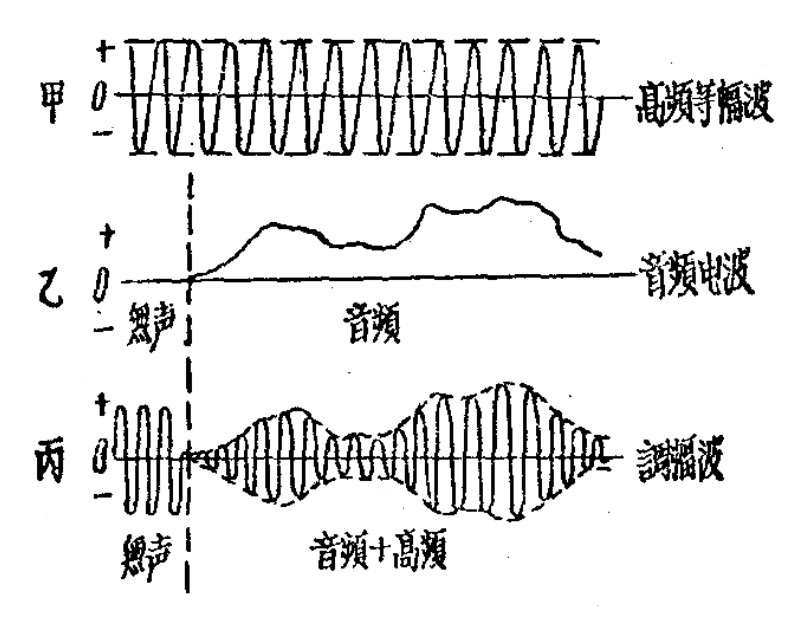
\includegraphics[width=0.9\textwidth]{am_modulation.jpg}
	\framebox[0.9\textwidth]{\parbox{0.85\textwidth}{\centering\vspace{3cm}AM调制波形示意图\\（自上而下：音频信号 → 载波 → 调幅波）\vspace{3cm}}}
	\caption{调幅（AM）调制过程波形示意}
	\label{fig:am_modulation}
\end{figure}

\textbf{类比总结}：

\begin{center}
\begin{tabular}{|c|c|c|}
	\hline
	\textbf{物理概念} & \textbf{类比对象} & \textbf{特点} \\
	\hline
	音频信号 & 货物 & 频率低、含信息、不能自行远传 \\
	\hline
	载波 & 运输卡车 & 频率高、无信息、可高效发射 \\
	\hline
	调制过程 & 装货上车 & 将货物装载到卡车上 \\
	\hline
	已调制波 & 满载的卡车 & 携带信息且能有效传播 \\
	\hline
	检波/解调 & 卸货 & 从已调制波中取出原始音频 \\
	\hline
\end{tabular}
\end{center}

\subsection{高频电流与电磁波的产生}

需要特别指出的是，直流电和低频交流电并不能有效地辐射电磁波。只有当电流的频率足够高时，才能实现有效的电磁辐射。这是因为电磁辐射的效率与频率的四次方成正比（根据经典电动力学理论），频率越高，辐射效率越显著。

当高频电流被输送到发射天线后，便会在周围空间激发起向外传播的电磁波。这一过程的物理机制可描述如下：

\begin{enumerate}
	\item \textbf{电场的产生}：高频电流在导线中流动时，导线上分布着随时间变化的电荷。这些变化电荷在导线周围激发出变化的\textbf{电场}。
	
	\item \textbf{磁场的产生}：根据安培定律，变化的电场会在其周围诱导出变化的\textbf{磁场}。
	
	\item \textbf{相互耦合传播}：变化的磁场又会根据法拉第电磁感应定律产生新的变化电场；新产生的变化电场再次诱发新的变化磁场……如此循环往复，形成电场→磁场→电场→磁场……的连续交替过程。
	
	\item \textbf{垂直关系}：在这一过程中，电场方向、磁场方向以及电磁波的传播方向三者两两互相垂直，构成右手螺旋关系。
	
	\item \textbf{向外扩散}：这种电磁振荡像一根根连续的链条，以光速向四面八方蔓延扩张——这就是\textbf{电磁波}的传播过程。
\end{enumerate}

简而言之：\textbf{变化的电场产生磁场，变化的磁场又反过来产生电场}，两者相互激发、相互依存，共同构成了能够在真空中独立传播的电磁波。

对于无线电广播而言，发射天线中的载波频率通常在数百千赫兹至数百兆赫兹范围，远高于工频交流电（50/60 Hz），因此能够高效地向空间辐射电磁波。

\subsection{波长及其计算}

电磁波在传播过程中，除了用频率来描述其振荡快慢外，还可以用另一个重要物理量——\textbf{波长}来表征。

\subsubsection{波长的定义}

\textbf{波长}（Wavelength）是指电磁波在一个完整周期内传播的距离，即波形中两个相邻的同相位点（如相邻的两个波峰或波谷）之间的距离。常用希腊字母$\lambda$（lambda）表示。

形象地说：如果电磁波是水面上的一圈圈涟漪，那么波长就是相邻两圈波纹之间的间距。\subsubsection{波长的计算公式}

电磁波以光速$c$在真空中（或近似地在空气中）传播。因此，波长$\lambda$、频率$f$与传播速度$c$三者之间存在如下关系：

\begin{equation}
	\lambda = \frac{c}{f}
\end{equation}

其中：
\begin{itemize}
	\item $\lambda$ —— 波长，单位为米(m)
	\item $c$ —— 光速，真空中约为 $2.998 \times 10^{8}$ m/s（工程上常取 $3 \times 10^{8}$ m/s）
	\item $f$ —— 频率，单位为赫兹(Hz)
\end{itemize}

由此公式可知：\textbf{频率越高，波长越短；频率越低，波长越长}。\subsubsection{实际应用举例}\begin{table}[htbp]
	\centering
	\caption{常见无线电频段的波长对照表}
	\label{tab:wavelength_examples}
	\begin{tabular}{llll}
		\hline
		\textbf{频段名称} & \textbf{频率范围} & \textbf{波长范围} & \textbf{典型应用} \\
		\hline
		中波(MW)   & 530--1700 kHz  & 约176--566 m & AM广播 \\
		短波(SW)   & 3--30 MHz      & 约10--100 m  & 远距离广播、业余电台 \\
		调频(FM)   & 88--108 MHz    & 约2.8--3.4 m & 调频广播 \\
		\hline
	\end{tabular}
\end{table}

以我国常用的中波广播频率1000 kHz（即1 MHz）为例：
\begin{align*}
	\lambda &= \frac{3 \times 10^{8} \text{ m/s}}{1 \times 10^{6} \text{ Hz}} = 300 \text{ m}
\end{align*}
也就是说，这个频率的无线电波的波长约为300米——大约相当于三个标准足球场的长度！

而对于调频广播频率98 MHz：
\begin{align*}
	\lambda &= \frac{3 \times 10^{8} \text{ m/s}}{98 \times 10^{6} \text{ Hz}} \approx 3.06 \text{ m}
\end{align*}
波长仅约3米左右，远短于中波。\subsubsection{波长对天线设计的影响}

了解波长对于无线电接收设备的设计具有重要意义。一般而言，天线的最佳长度与波长相关：

\begin{itemize}
	\item \textbf{半波天线}：长度约为$\lambda/2$，是最常见的高效天线形式
	\item \textbf{四分之一波长天线}：长度约为$\lambda/4$，常用于便携式设备
\end{itemize}

这也是为什么矿石收音机需要较长的天线来有效接收中波信号——因为中波波长可达数百米，即使使用四分之一波长天线也需要数十米的导线长度。

\section{接收无线电波的方法}

\subsection{天线接收原理}

在电台电磁波所能覆盖的范围内，架设一根金属导线（称为\textbf{接收天线}，或简称\textbf{天线}），当电台发射的电磁波传播至该导线时，由于电磁感应作用，导线上会产生与发射天线上相似的高频电流。

这一过程的物理本质是\textbf{电磁感应}：变化的电磁场会在导体中感应出电动势，从而驱动电荷定向移动形成电流。所产生的感应电流频率与入射电磁波的载波频率相同，但其幅度则取决于多种因素：

\begin{itemize}
	\item \textbf{天线长度}：当天线长度与波长匹配（如半波或四分之一波长）时，接收效率最高
	\item \textbf{电磁波强度}：距离发射台越远，信号越弱
	\item \textbf{天线取向}：对于线极化波，天线方向与电场方向一致时效果最佳
	\item \textbf{周围环境}：建筑物、地形等会对电磁波产生反射、吸收和遮挡效应
\end{itemize}

\subsection{信号的引入与传输}

天线接收到的高频感应电流，通过一根与天线相连接的\textbf{引线}（又称\textbf{馈线}或\textbf{引入线}）传导至接收机输入端。这条引线起到了以下关键作用：

\begin{enumerate}
	\item \textbf{能量传递}：将天线上感应的高频电能无损（或低损耗）地输送至接收机
	\item \textbf{阻抗匹配}：良好的引线设计可实现天线与接收机之间的阻抗匹配，最大限度地减少信号反射和功率损失
	\item \textbf{噪声抑制}：合理布线的引线可降低对外部干扰的拾取
\end{enumerate}

对于矿石收音机这类简单的接收装置，引线通常是一根普通的绝缘铜导线即可满足需求；而对于更复杂的接收系统，则需要使用特性阻抗固定的同轴电缆或平行双线作为馈线。

\section{调谐电路——从众多电波中选出目标电台}

\subsection{选频的必要性}

天线接收到的并非单一电台的信号，而是空间中所有正在广播的电磁波的总和——包含中波、短波、调频等各个频段的无数电台信号混杂在一起。要从中选出我们所需的目标电台的信号，就必须使用一种称为\textbf{调谐电路}（又称\textbf{选频电路}或\textbf{谐振电路}）的装置。

\subsection{LC调谐电路的基本构成}

调谐电路通常由以下两个元件组成：

\begin{itemize}
	\item \textbf{电感线圈}（Inductor / Coil）：用绝缘导线绕制成的螺旋状线圈，具有储存磁场能量的特性，其电感量常用 $L$ 表示，单位为亨利(H)
	\item \textbf{可变电容器}（Variable Capacitor）：由两组金属极板构成，其中一组可以转动以改变极板间的相对面积，从而改变电容值。电容量常用 $C$ 表示，单位为法拉(F)
\end{itemize}

这两个元件连接在一起便构成了一个\textbf{LC串联谐振电路}，其固有谐振频率为：

\begin{equation}
	f_0 = \frac{1}{2\pi\sqrt{LC}}
\end{equation}

\subsection{调谐的工作原理}

当LC电路的固有频率 $f_0$ 与某个电台的载波频率一致时，该电路对该频率信号的阻抗最小（串联谐振时理论阻抗为零），使得该频率的电流能够顺利通过；而对于其他频率的信号，电路呈现较高的阻抗，使其难以通过——这就是所谓的\textbf{选频}或\textbf{滤波}作用。

通过调节可变电容器的容量（或改变线圈的电感量），可以改变电路的固有谐振频率 $f_0$，从而在众多电台中"锁定"目标频率。这一操作就是我们日常所说的"\textbf{调台}"或"\textbf{选台}"。

\subsection{调谐电路的局限性}

需要特别说明的是，调谐电路的选频能力是有局限性的：

\begin{itemize}
	\item \textbf{同频干扰}：如果两个电台的载波频率完全相同或极为接近，超出了调谐电路的分辨能力，则电路无法将它们分开，收音机中会同时听到两个节目混在一起的现象
	\item \textbf{选择性}：调谐电路区分相邻频率的能力称为"选择性"，它取决于电路的品质因数$Q$值。$Q$值越高，选择性越好，但通频带也越窄
	\item \textbf{邻频干扰}：强信号电台可能对其相邻频率的弱信号电台产生压制效应
\end{itemize}

正因如此，无线电频率管理部门会对每个广播电台分配互不相同的\textbf{工作频率}，且相邻电台之间需留有足够的频率间隔（保护频带），以免相互干扰。

\section{矿石收音机的基本原理}

矿石收音机利用天然矿石（如方铅矿、黄铁矿等）作为检波器，将调谐电路接收到的高频无线电信号转换为音频信号，通过耳机播放。它不需要电源，完全依靠天线接收到的无线电波能量工作。

\subsection{检波的必要性}

电台选定后，它的电流仍然是带有音频信号的高频电流，我们的耳朵无法感知叠加在上面的音频信号，必须经过一种装置，把载在高频电流上面的音频电流"检"出来。这个工作叫做"检波"（又称解调），由"检波器"来完成。

\subsection{矿石检波器的工作原理}

在矿石收音机里，检波器就是一块只让电流单方向通过的"矿石"或叫"晶体"。高频电流通过它时，只有一个方向的电流能够通过，反方向的电流就被阻止。经过检波以后，剩余的主要是音频电流及少量残余高频载波成分（通常需要通过滤波电路进一步去除）。

这一过程的本质是利用了矿石的\textbf{单向导电性}。当高频调幅信号通过矿石时：
\begin{itemize}
	\item 正半周电流能够通过
	\item 负半周电流被阻挡
\end{itemize}
这样就将高频载波的"包络"（即音频信号）提取出来，实现了从高频调幅波中还原音频信号的目的。

\subsection{音频信号的还原与收听}

音频电流很容易把它还原成为人耳所能听闻的声音——空气的振动。只要将它通过"耳机"（又称听筒、受话器），耳机里的磁力便会依着音频电流的变化吸动它的振膜，将电流的振动变成机械振动，激荡空气成为声音。

\chapter{矿石收音机的天线系统}

天线是矿石收音机接收无线电信号的关键部件，其性能直接影响收音效果。良好的天线系统是矿石收音机正常工作的基础。

\section{天线的作用与要求}

天线是收音机接收电磁波的前端部件，其作用是将空间中的电磁波转换为感应电流。当天线长度与接收信号的波长可比拟时，能产生显著的谐振效应，从而获得最大的感应电动势。

天线的接收效率主要取决于以下因素：
\begin{itemize}
	\item \textbf{长度}：在一定范围内，天线越长，感应的信号能量越强。但过长的天线会增加架设难度并可能引入更多干扰。
	\item \textbf{高度}：架设位置越高，越能避开地面障碍物的遮挡和地面反射波的干扰，接收效果越好。
	\item \textbf{环境}：天线周围的建筑物、树木等会对电波产生阻挡和反射，影响接收效果。开阔地带的接收条件优于密集城区。
\end{itemize}

对于中波接收，矿石收音机的天线长度通常在20-30米之间，架设高度离地面10-20米即可获得较好的接收效果。实际架设时需根据当地电台信号强度和环境条件进行调整。

\section{天线的结构型式}

天线通常由两部分组成：一根悬挂在空中的金属导线（称为"天线振子"）和一根连接振子与接收机的"引入线"（又称馈线）。常见的天线架设型式有两种：

\begin{itemize}
	\item \textbf{Γ型天线}：引入线从天线振子的一端引出，整体形状类似希腊字母Γ（Gamma）
	\item \textbf{T型天线}：引入线从天线振子的中点引出，整体形状类似字母T
\end{itemize}

这两种型式的天线在接收效果上基本相同，主要区别在于引入线与天线振子的连接位置。它们的共同优点是结构简单、架设方便，适合矿石收音机使用。

\section{天线的绝缘要求}

天线的水平部分（振子）不能直接绑在杆子上，否则会导致接收到的信号能量通过杆子泄漏——尤其在潮湿或下雨时，泄漏更为严重。因此，导线的两端必须使用"绝缘子"与支撑物隔开。

\textbf{绝缘的作用}：绝缘就是阻止电流通过的意思。在无线电设备中，很多地方需要用绝缘材料将不同电位的导体分隔开，以防止漏电或短路。常见的绝缘材料包括玻璃、陶瓷、橡胶等。

\textbf{绝缘子的安装}：绝缘子的一端用铁丝固定在支撑物上，另一端连接天线。需要特别注意的是，固定用的铁丝不能与天线导线直接接触，否则会造成短路，导致信号能量损失。

\textbf{天线的拉紧与松紧调整}：天线两端绝缘子的高度不一定要相等，但天线必须拉紧以保持平直。为方便调整天线松紧，可在支撑物的一端安装一个小滑轮，通过拉线来调节。需要注意的是，天线不宜拉得太紧，否则在寒冷天气时，导线会因热胀冷缩而收缩，可能导致导线或支撑物被拉断。

\textbf{天线安装的注意事项}：架设天线时，应根据具体环境灵活安排，需特别注意以下几点：

\begin{enumerate}
	\item \textbf{足够的高度和长度}：确保天线有足够的高度和长度，以接收更多的信号能量。
	\item \textbf{良好的绝缘}：确保所有绝缘部位性能良好，防止信号泄漏。
	\item \textbf{坚固安全}：天线及其支撑结构必须坚固可靠，确保使用安全。
\end{enumerate}

此外，天线和引入线应尽量远离电力线（如电灯线），更不要跨越它们。这样可以防止天线意外折断时与电力线接触，避免发生触电危险。

\section{天线导线的材料与规格}

天线的导线应选用导电性良好的材料，通常使用多股绞合铜线。多股绞合线的优点是表面积较大，高频电流的集肤效应使其能够获得更多的信号电流，能量损失较小。

除了专用的多股天线线外，直径1.5-2.5毫米的单根铜线也可使用。此外，现成的胶皮铜线、电灯花线等绝缘电线也能作为天线使用。用作天线时，外面的绝缘层（如胶皮、棉纱套等）不必剥去，因为电磁波能够穿透这些绝缘物质，不会影响收音效果。

这类电线同样适合用作引入线。但在天线与引入线的连接处，必须确保连接牢固且接触良好，以减少信号损耗。

\section{接收距离的限制}

矿石收音机的接收距离受多种因素制约：
\begin{itemize}
	\item \textbf{电台功率}：发射功率越大，覆盖范围越广。
	\item \textbf{传播条件}：中波主要依靠地波传播，受地形、地电特性影响较大。
	\item \textbf{天线性能}：天线的有效高度和效率直接影响信号接收能力。
\end{itemize}

当接收地点距离电台较远时，即使使用高性能天线，信号强度也会显著衰减。若此时使用质量较差的天线，接收效果将进一步恶化，可能无法正常收听。

\chapter{矿石收音机的地线系统}

地线是矿石收音机天地线系统的重要组成部分，它与天线共同构成一个完整的高频回路。地球作为一个巨大的导体，可以看作是高频电流的返回路径。对于无源的矿石收音机来说，良好的接地同样是获得良好收音效果的关键。

\section{地线的作用与要求}

连接地线的主要作用是：
\begin{itemize}
	\item \textbf{形成完整回路}：为高频信号提供返回路径，使天线接收到的信号能够形成完整的电流回路。
	\item \textbf{提高接收效率}：良好的接地可以显著提高矿石收音机的灵敏度和选择性，使收音效果更好。
	\item \textbf{稳定信号}：地线可以起到一定的屏蔽作用，减少外界干扰。
\end{itemize}

\section{地线的安装方法}

地线的关键是要与地面紧密接触。常见的安装方法有：

\begin{itemize}
	\item \textbf{螺旋埋设法}：将导线末端卷成数圈螺旋形，直接埋入地下。
	\item \textbf{金属辅助法}：将导线缠绕在铁棒或铜块上，然后一起打入地里。
\end{itemize}

\section{地线的埋设要求}

\textbf{埋置地点的选择}：应选择潮湿、土质较为黏稠的泥土作为接地位置。干燥的砂地导电性很差，不宜作为接地点。埋设深度一般在60厘米（约二尺）以下即可。

\textbf{城市环境中的接地方法}：在城市中，可以利用自来水管或暖气片作为地线，因为它们都有一部分埋在地下，导线接在上面即可实现接地。但需注意：
\begin{itemize}
	\item \textbf{禁止使用煤气管道}：为防止危险，煤气管道严禁用作地线。
	\item \textbf{确保良好接触}：这些管道外面通常有油漆或积垢，接线前需用锉刀将接触面打磨干净，然后将导线紧密缠绕几圈并绞紧，最好采用焊接方式确保接触良好。
\end{itemize}

\chapter{矿石收音机的调谐线圈}

线圈是矿石收音机调谐电路中的核心元件，它与可变电容器配合构成LC谐振电路，实现对不同频率电台的选择。

\section{线圈的结构与制作}

简单收音机中的线圈，通常是用外面包有绝缘层的铜线密排地绕在绝缘质的圆筒上，或者绕在有辐射状长齿的纸板上。常用的绝缘材料包括纸筒、胶木筒等。

\textbf{线圈骨架的选择}：矿石收音机的线圈采用直径较大的圆筒式骨架效率比较好。但圆筒直径也不宜过大，否则会使收音机的体积变得过于庞大。适宜的圆筒直径通常在30-70毫米之间。

\textbf{绕线方法}：绕线前应先将线头固定在纸筒（线圈管）上。在开始的地方用针刺两个小孔，将线穿过两孔绕一圈，线就固定下来了（参见图 \ref{fig:coil-termination}）。线端留出80-100毫米的长度作为接线用。绕在纸筒上的导线要排列整齐、紧贴，使线圈绕好后不会松动。

\begin{figure}[htbp]
	\centering
	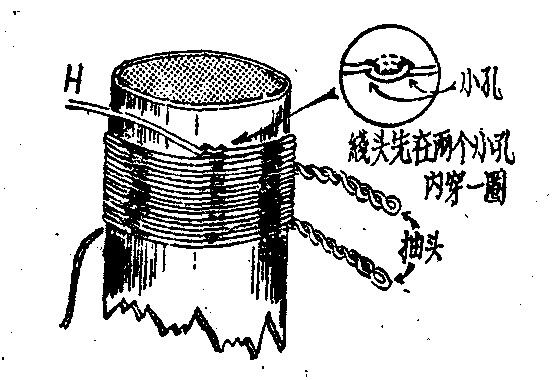
\includegraphics[width=0.8\textwidth]{coil-termination-method.jpg}
	\caption{线圈线头固定方法示意图}
	\label{fig:coil-termination}
\end{figure}

\textbf{抽头的制作}：对于需要通过增减圈数来调整电感量的调谐线圈，需要在适当的圈数上抽出抽头，以便获得不同的电感值。抽头数量通常较多，需根据电路图的说明每隔多少圈抽一个头。绕到指定抽头的圈数时，将导线引出打一个折，长度约30毫米，从折合端开始绕转绞合起来，到纸筒边缘为止。抽头不要剪断，可继续绕下去；抽头时要左右看齐，使线圈绕好后所有抽头都能排成一行整齐的行列。抽头的末端都要将绝缘漆（或包纱）刮去至金属闪亮，准备接线。

\section{线圈的电感特性}

导线绕成线圈后就具有"电感"——对交流电流发生特殊效应的现象。同一电感量的线圈，对不同频率的交流电流有不同的阻碍作用。

电路里常利用电感量的变更来调谐电台的频率，选择需要的电波而将不需要的加以剔除。电感与电容配合形成的谐振电路，其谐振频率公式为：
\[ f_0 = \frac{1}{2\pi\sqrt{LC}} \]
其中，\( f_0 \)为谐振频率，\( L \)为电感，\( C \)为电容。通过改变线圈的电感量或电容器的电容量，即可改变谐振频率，从而实现选台功能。

\section{影响电感量的因素}

线圈的电感量与多种因素有关，包括：
\begin{itemize}
	\item \textbf{线圈长度}：线圈越长，电感量越大。
	\item \textbf{圆筒直径}：线圈骨架直径越大，电感量越大。
	\item \textbf{导线粗细}：导线直径对电感量影响较小，但会影响线圈的Q值和损耗。
	\item \textbf{绕制方式}：线圈的绕制型式和疏密程度也会影响电感量。
\end{itemize}

在实际应用中，通常通过改变线圈的圈数来调整电感量。不同的波段需要不同电感量的线圈，例如中波广播段需要的电感量通常在几十到几百微亨之间。

\section{绕制线圈用的导线}

绕制线圈的导线必须具有良好的绝缘层，以确保各圈之间不会短路。常用的导线类型有：

\begin{itemize}
	\item \textbf{漆包线}：外面涂有绝缘漆的铜线。即使线圈绕得很紧密，漆层也能保证每圈之间的电气隔离，不会发生漏电。因此，裸铜线不能用于绕制这类线圈。
	\item \textbf{纱包线}：用纱线包裹的导线，同样具有良好的绝缘性能。
	\item \textbf{丝包线}：用丝线包裹的导线，常用于要求较高的场合。
\end{itemize}

\textbf{导线的线径选择}：选择适宜线径的导线，才能得到良好的效果。导线的粗细用"线规"来表示，线规有很多种规格标准，我国使用的规格称为"中规"，直接以线的直径来表示。

矿石收音机线圈常用的导线规格为中规0.31号、0.45号、0.56号等（它们的直径分别是0.31毫米、0.45毫米、0.56毫米）。如果使用其他规格标准的导线，只要直径相同也可以适用。

\section{多线圈的绕制注意事项}

在矿石收音机电路中，有时会使用两个或多个线圈。除非电路图特别说明采用特殊绕制方法，否则通常的做法是：

\begin{itemize}
	\item \textbf{同筒绕制}：将两个线圈绕在同一个圆筒上；
	\item \textbf{嵌套绕制}：将一个线圈绕在较小的纸筒上，然后套入另一个较大纸筒内的线圈中。
\end{itemize}

无论采用哪种方式，都需要注意以下几点：
\begin{itemize}
	\item \textbf{绕线方向一致}：两个线圈的绕线方向必须相同，否则会产生相互抵消的磁场，影响电路正常工作；
	\item \textbf{分清线头线尾}：接线时必须按照电路图的说明分清每个线圈的首尾端（通常标记为头/尾或始/末）；
	\item \textbf{正确连接}：如果接错线头，线圈之间的耦合会失效，电路将无法正常工作。
\end{itemize}

\backmatter

\end{document}
